% !TeX root = ../pythonTutorial.tex
\chapter{Interpolation}

Die Interpolation betrifft die Werte f�r die Versuche im Elektrolabor. \newline

Das Problem hier war die Beschaffung der Formeln zur Berechnung m�glichst realistischer Werte. Die f�r den Moment einfachste Variante schien, uns die reellen Zahlen in einen Graph umzuwandeln und zu schauen, welche Funktion m�glichst nah ran kommt.

Die Interpolation einer halbwegs passenden Funktion gestaltete sich recht schwierig. Wir hatten Daten-Tabellen in folgender Form als Vorgabe:

\begin{table}[]
	\begin{tabular}{lllll}
		Ur    &          &  & Uc    &          \\
		Input & Ergebnis &  & Input & Ergebnis \\
		&          &  &       &          \\
		15    & 0,3      &  & 15    & 4        \\
		20    & 0,5      &  & 20    & 4        \\
		30    & 0,7      &  & 30    & 3,9      \\
		50    & 1,2      &  & 50    & 3,8      \\
		70    & 1,6      &  & 70    & 3,7      \\
		100   & 2,1      &  & 100   & 3,4      \\
		150   & 2,7      &  & 150   & 2,9      \\
		300   & 3,5      &  & 300   & 1,9      \\
		700   & 3,8      &  & 700   & 0,9      \\
		1000  & 3,9      &  & 1000  & 0,6      \\
		1500  & 3,9      &  & 1500  & 0,4      \\
		2000  & 3,9      &  & 2000  & 0,3     
	\end{tabular}
\end{table}

Um die Daten in einen Funktionsgraphen inklusive passender Funktion umzuwandeln wurde MyCurveFit(\cite{MyCurveFit}) benutzt. Die Daten wurden in Tabellenform hochgeladen und dann wurde die Funktion genommen, die am besten gepasst hat.

\begin{figure}
	\centering
	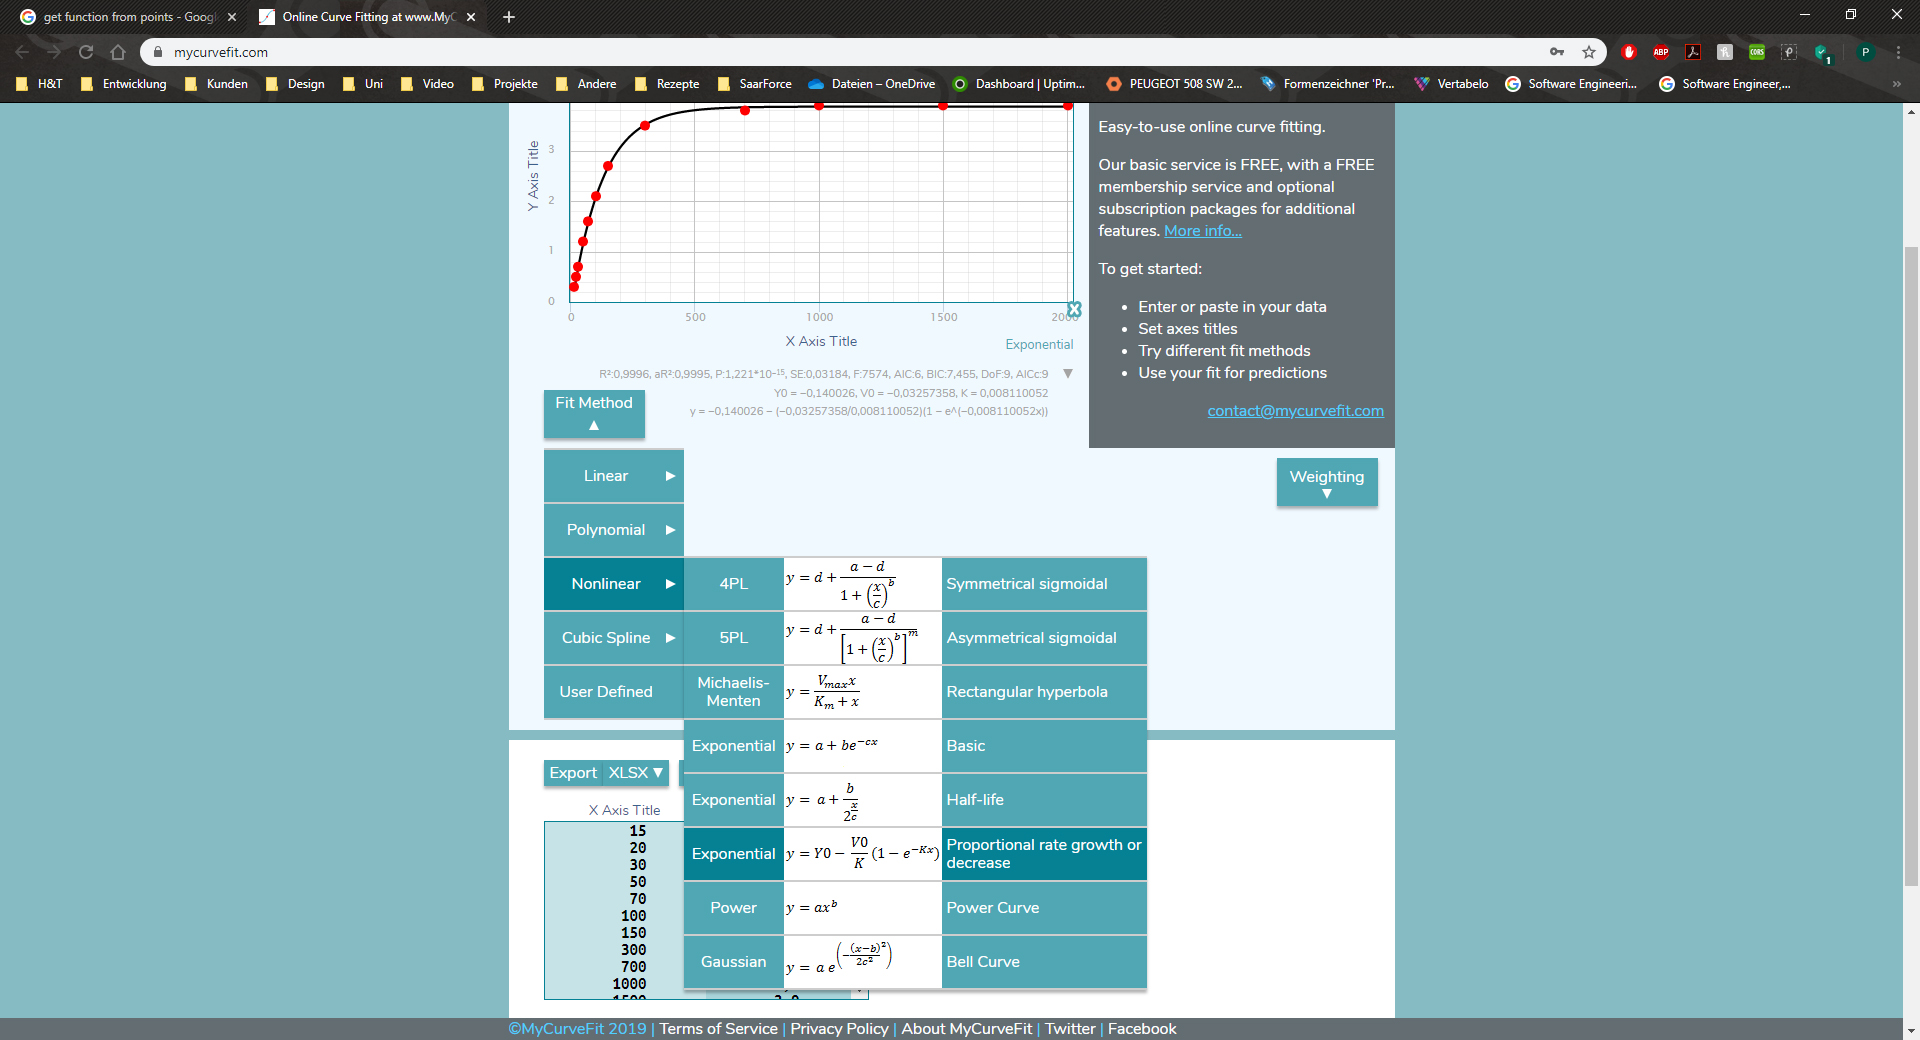
\includegraphics[width=1\textwidth]{images/interpolation/beispiel_online_fitting.jpg}
	\caption{MyCurveFit Website mit Beispiel Funktion}
	\label{img:mycurvefit}
\end{figure}

\begin{figure}
	\centering
	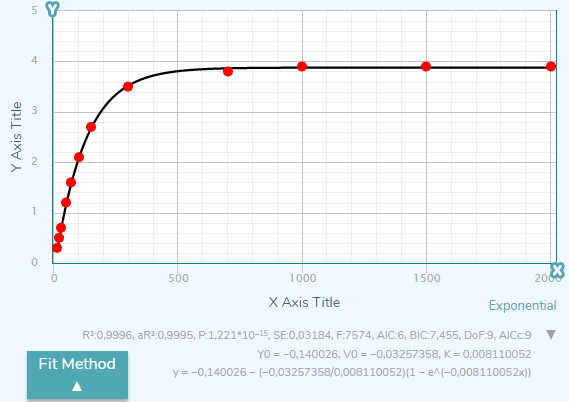
\includegraphics[width=0.8\textwidth]{images/interpolation/graph_uc.png}
	\caption{Funktionsgraph Uc}
	\label{img:graphuc}
\end{figure}

\begin{figure}
	\centering
	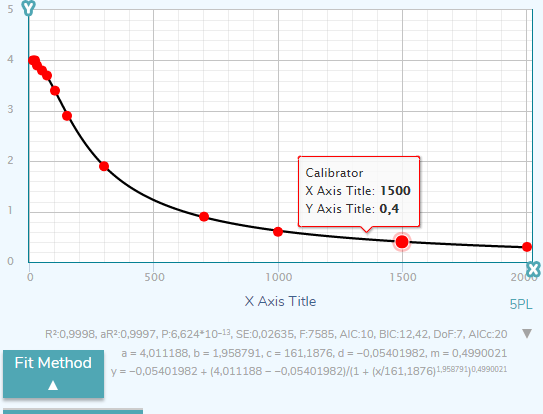
\includegraphics[width=0.8\textwidth]{images/interpolation/graph_ur.png}
	\caption{Funktionsgraph Ur}
	\label{img:graphur}
\end{figure}
